\documentclass[10pt]{article}

\usepackage{amsmath}
\usepackage{booktabs}
\usepackage{geometry}
\usepackage{graphicx}
\usepackage{hyperref}
\usepackage{multirow}
\usepackage{enumitem}
\usepackage{xcolor}
\usepackage{caption}

\geometry{margin=1.6cm}
\setlength{\parskip}{0.35em}
\setlength{\parindent}{0pt}
\setlist[itemize]{leftmargin=1.3em, itemsep=0.1em, topsep=0.2em}
\captionsetup{font=small, labelfont=bf}
\raggedbottom

\title{\textbf{Data to Design: Machine Learning Report}\\\large Linear Model Family}
\author{S1 Linear Family}
\date{July 2026}

\begin{document}
\maketitle
\pagenumbering{roman}
\tableofcontents
\newpage
\listoftables
\listoffigures
\newpage
\pagenumbering{arabic}

\section{Introduction}

\subsection{Engineering Problem}
Concrete strength prediction is useful because laboratory testing is slow and expensive. A model that estimates compressive strength from mix composition can help engineers compare designs before physical testing. This report studies two datasets: the UCI concrete dataset for standard concrete and the UHPC dataset for ultra-high-performance concrete.

\subsection{Scope of the Linear Model Family}
The assigned model family is linear regression and its regularized or expanded forms:
\begin{itemize}
    \item Ordinary Least Squares (OLS),
    \item Elastic Net,
    \item Bayesian Ridge,
    \item Polynomial Ridge.
\end{itemize}
The purpose is not only to get high accuracy, but also to understand where simple and interpretable models work well and where they fail.

\section{Data and Methodology}

\subsection{UCI Concrete Dataset}
The UCI concrete dataset contains eight input features: cement, slag, fly ash, water, superplasticizer, coarse aggregate, fine aggregate, and age. The target is compressive strength in MPa. The cleaned modeling file used here has 1005 complete and non-duplicate rows.

The baseline UCI experiment used an 80/20 train-test split. For model tuning, the baseline was corrected to use 4-fold cross-validation, following the four-part validation idea in Yeh's original concrete strength study. The representation experiments also used 4-fold cross-validation.

\subsection{UHPC Dataset}
The UHPC dataset started with 2188 rows. After keeping rows with a valid 28-day compressive strength target, 2073 rows remained. From the shared semantic 50\% representation, publication metadata was removed from the predictors so that the model could not directly learn paper identity.

\begin{table}[h!]
\centering
\small
\caption{UHPC shared semantic 50\% preprocessing summary.}
\label{tab:uhpc-preprocessing}
\begin{tabular}{lrrrr}
\toprule
\textbf{Dataset} & \textbf{Rows} & \textbf{Raw Predictors} & \textbf{Numeric} & \textbf{Categorical} \\
\midrule
Source data with publication & 2073 & 34 & 24 & 9 \\
Modeling data without publication & 2073 & 33 & 24 & 9 \\
Encoded model matrix & 2073 & 60 & -- & -- \\
\bottomrule
\end{tabular}
\end{table}

Numeric features were median-imputed and standardized. Categorical features were encoded using one-hot encoding for lower-cardinality columns and target encoding for higher-cardinality material descriptors. The target encoder used 5 internal folds inside the preprocessing pipeline.

\section{Results and Interpretation}

\subsection{UCI Concrete Results}

\begin{table}[h!]
\centering
\small
\caption{UCI Linear Family results on the 20\% test split.}
\label{tab:uci-results}
\begin{tabular}{llrrrr}
\toprule
\textbf{Representation} & \textbf{Best Model} & \textbf{MAE} & \textbf{RMSE} & \textbf{$R$} & \textbf{$R^2$} \\
\midrule
Original features & Polynomial Ridge & 4.69 & 6.57 & 0.929 & 0.862 \\
Domain ratios & Polynomial Ridge & 4.72 & 6.71 & 0.926 & 0.856 \\
Log-transformed features & Polynomial Ridge & 4.03 & 5.80 & 0.946 & 0.892 \\
Interaction features & Polynomial Ridge & 3.78 & 5.66 & 0.949 & 0.897 \\
\bottomrule
\end{tabular}
\end{table}

The ordinary linear models were not flexible enough for the UCI data. OLS, Elastic Net, and Bayesian Ridge stayed around RMSE 10.9 and $R^2 \approx 0.62$ on the original features. Polynomial Ridge performed much better because it can model curved relationships, especially the nonlinear effect of age and mix ratios.

The best result came from Polynomial Ridge with interaction features. Across three random seeds, this setting achieved RMSE $5.17 \pm 0.49$ and $R^2 = 0.901 \pm 0.007$, so the result was reasonably stable.

\begin{figure}[h!]
\centering
\begin{minipage}{0.48\textwidth}
    \centering
    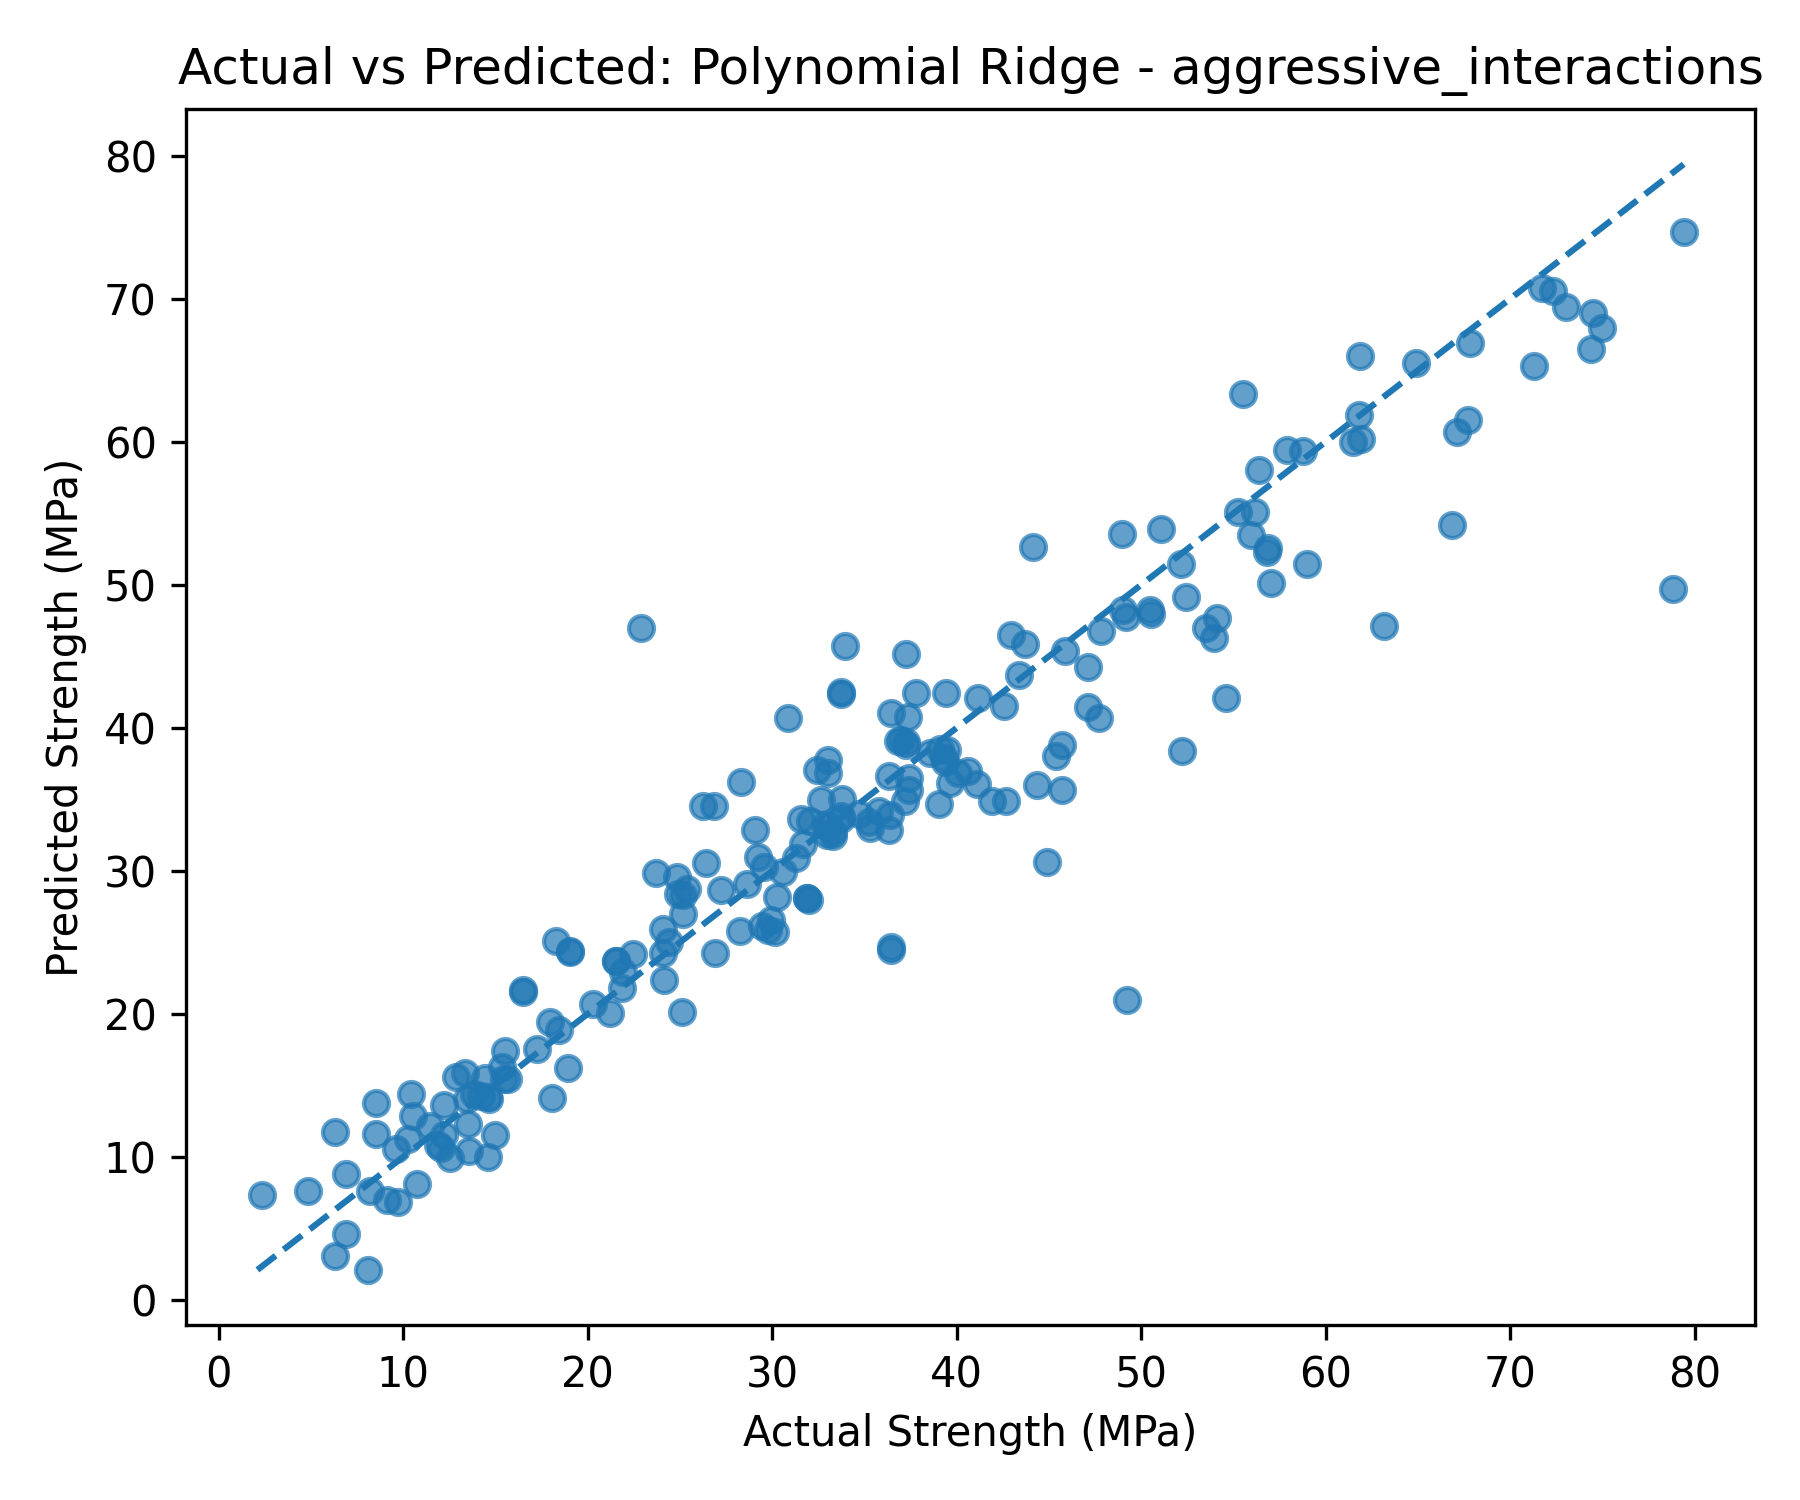
\includegraphics[width=\textwidth]{report_assets/uci_polynomial_actual_vs_predicted.png}
\end{minipage}
\hfill
\begin{minipage}{0.48\textwidth}
    \centering
    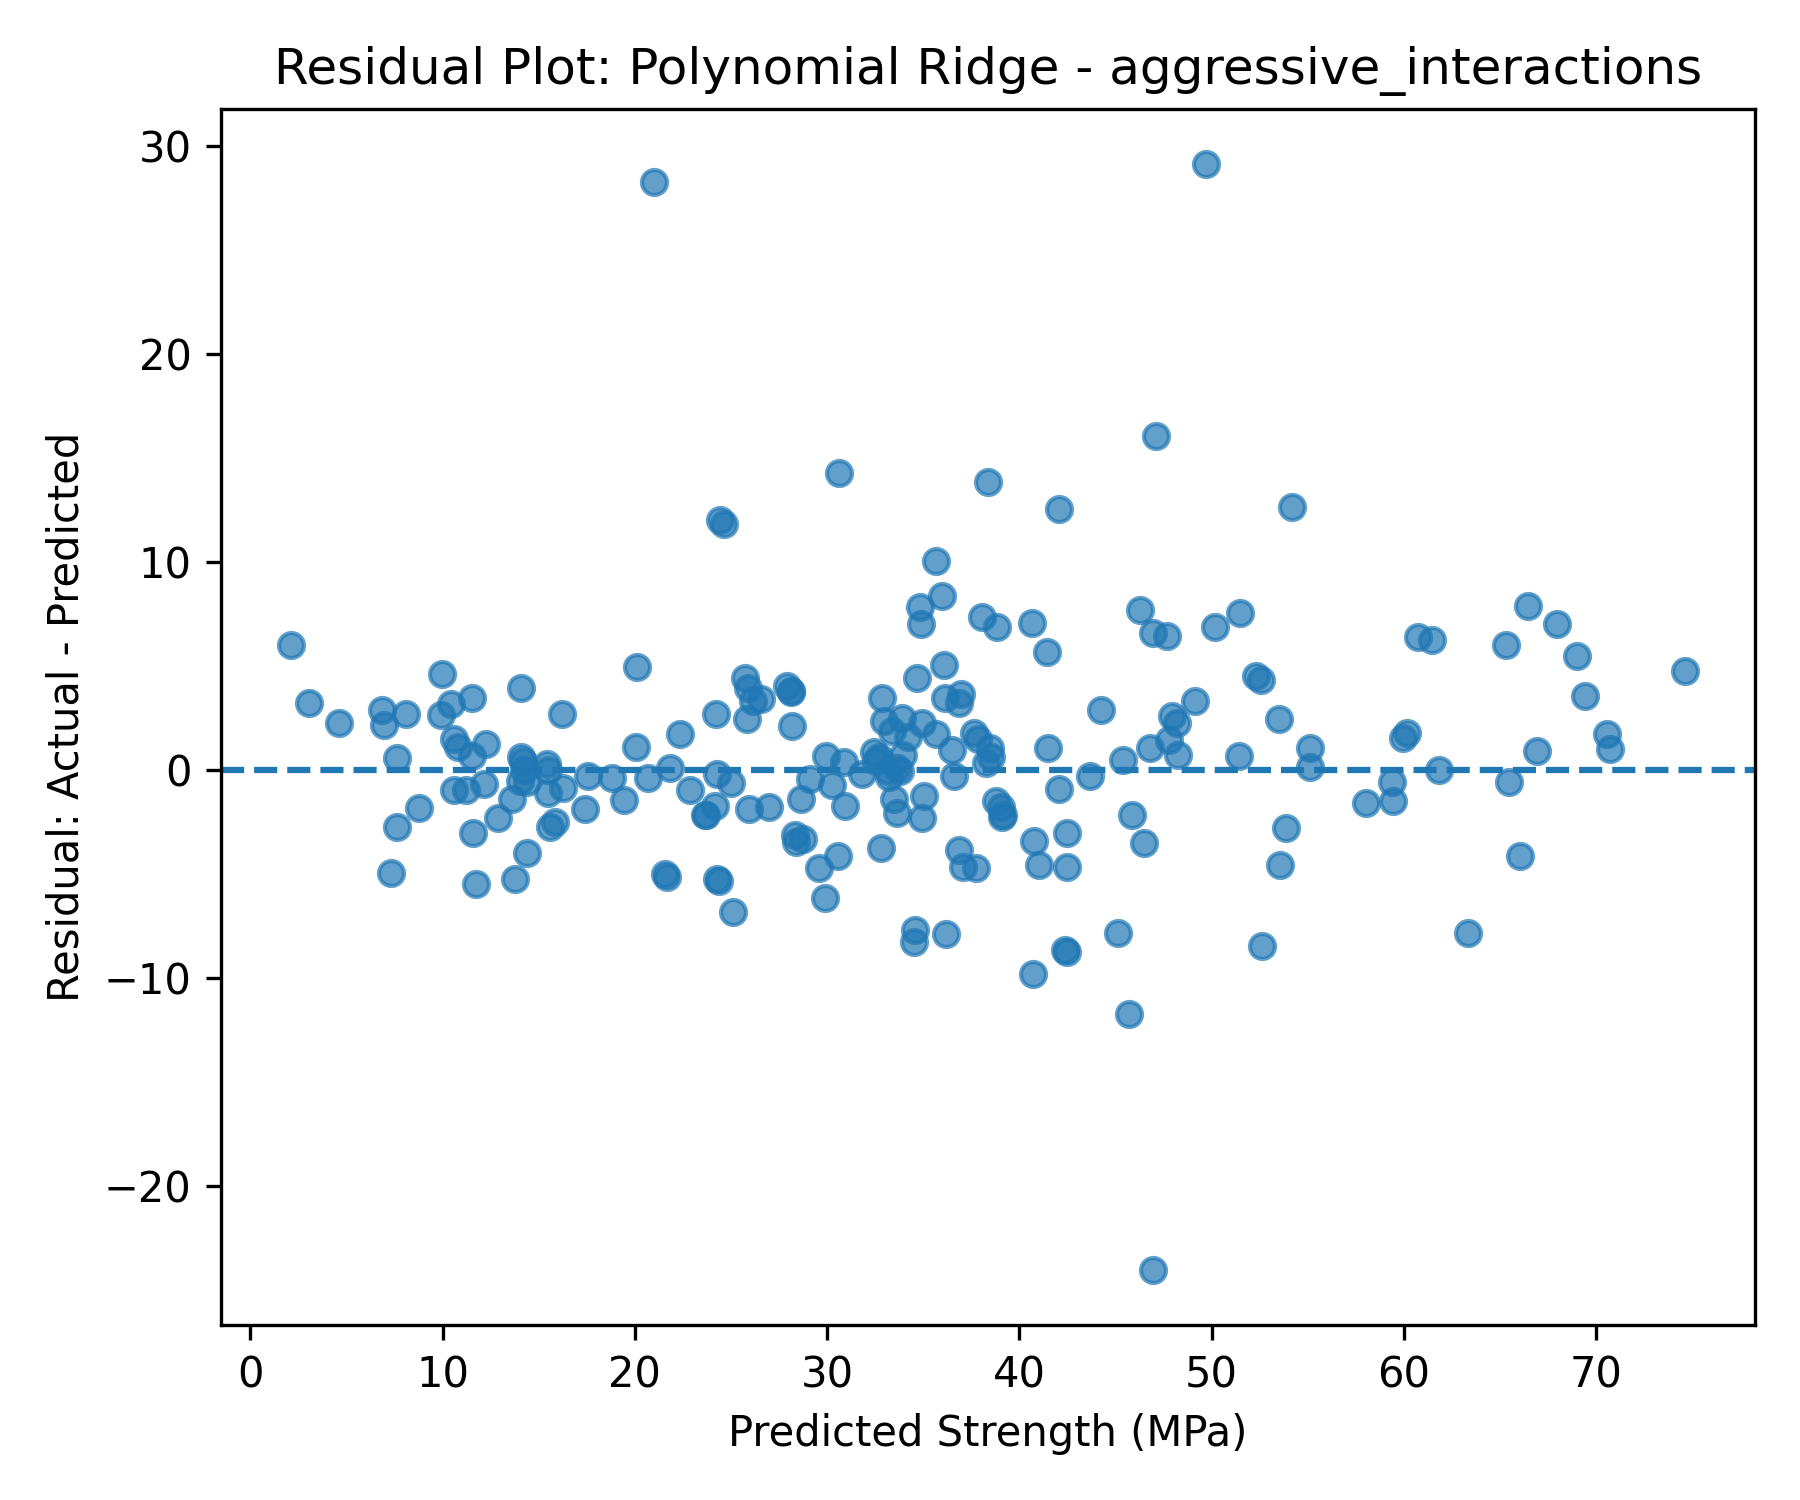
\includegraphics[width=\textwidth]{report_assets/uci_polynomial_residuals.png}
\end{minipage}
\caption{UCI Polynomial Ridge prediction behavior. The left plot compares actual and predicted strength; the right plot shows the residual pattern.}
\label{fig:uci-polynomial}
\end{figure}

\subsection{UHPC Row-Mixed Results}
The row-mixed UHPC split used a feature-hash grouped 70/15/15 strategy. The final sizes were 1449 training rows, 311 validation rows, and 313 test rows. The grouping prevented identical feature vectors from appearing in different splits.

\begin{table}[h!]
\centering
\small
\caption{UHPC row-mixed Linear Family performance.}
\label{tab:uhpc-rowmixed}
\begin{tabular}{lrrrrrr}
\toprule
\textbf{Model} & \multicolumn{3}{c}{\textbf{Validation}} & \multicolumn{3}{c}{\textbf{Test}} \\
\cmidrule(lr){2-4}\cmidrule(lr){5-7}
 & \textbf{MAE} & \textbf{RMSE} & \textbf{$R^2$} & \textbf{MAE} & \textbf{RMSE} & \textbf{$R^2$} \\
\midrule
OLS & 16.97 & 21.96 & 0.662 & 16.56 & 21.09 & 0.685 \\
Elastic Net & 16.98 & 21.75 & 0.669 & 16.54 & 20.91 & 0.690 \\
Bayesian Ridge & 16.99 & 21.74 & 0.669 & 16.56 & 20.93 & 0.689 \\
Polynomial Ridge & 30.65 & 343.34 & -81.54 & 11.14 & 15.51 & 0.829 \\
\bottomrule
\end{tabular}
\end{table}

Bayesian Ridge was selected because it had the lowest validation RMSE among the stable models. Polynomial Ridge had a strong test score, but its validation error was extremely unstable. Therefore, it was not treated as the main UHPC model.

The targeted checks were useful. Removing fiber features increased Elastic Net test RMSE from 20.91 to 23.94, so fiber information clearly helped. Removing training outliers also made performance worse, increasing Elastic Net test RMSE to 22.35. Extra engineering ratios did not improve the linear models.

\begin{figure}[h!]
\centering
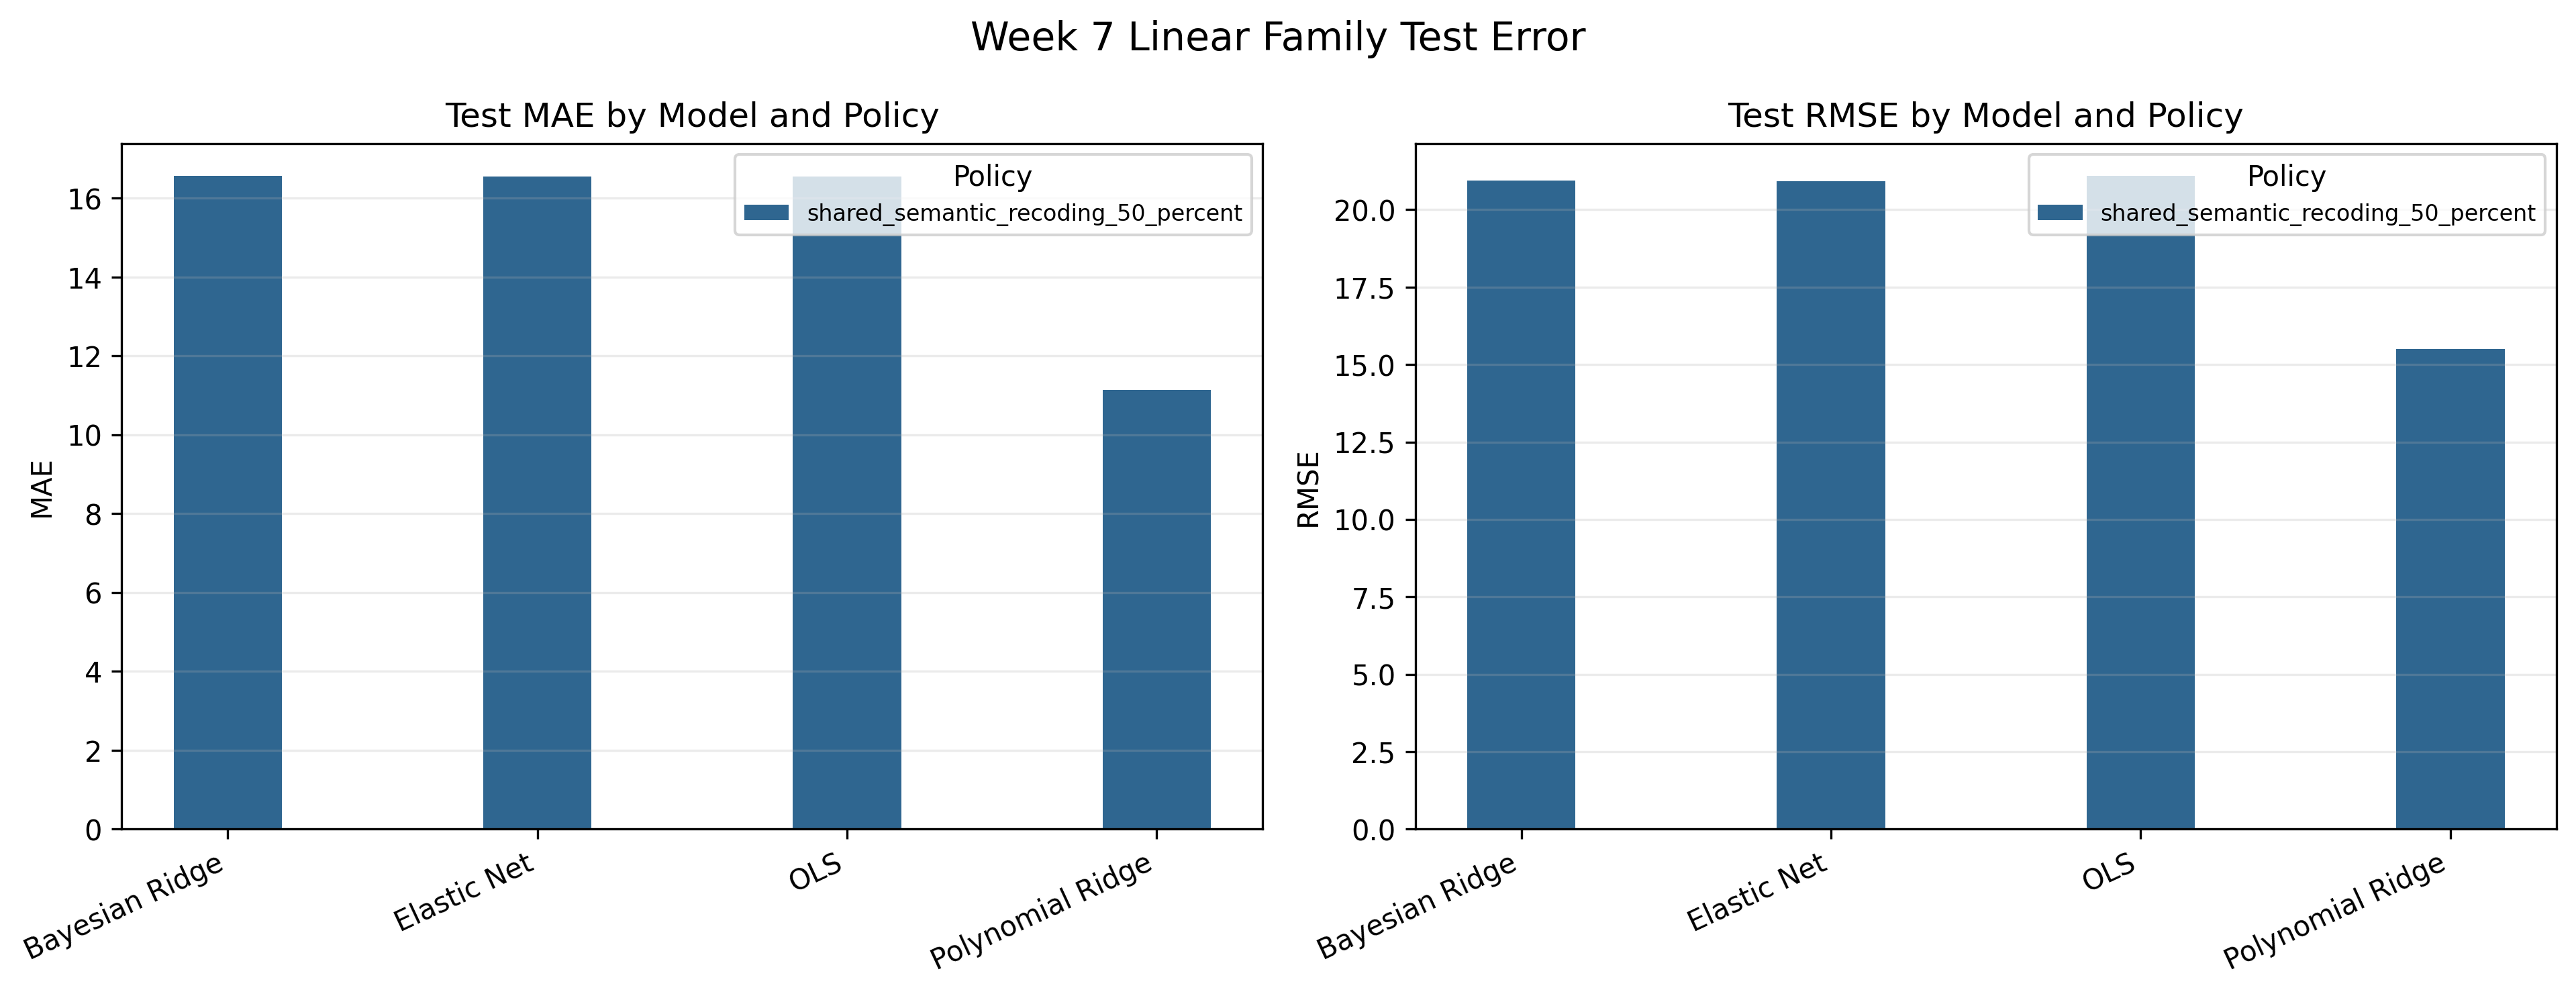
\includegraphics[width=0.92\textwidth]{report_assets/uhpc_row_mixed_metrics.png}
\caption{Row-mixed UHPC metric comparison across the Linear Family models.}
\label{fig:uhpc-rowmixed}
\end{figure}

\subsection{Publication Generalization}
Row-mixed testing can be optimistic because rows from the same publication may share experimental habits, equipment, and mix-design style. To test generalization more honestly, we held out complete publications. This split used 115 training publications, 25 validation publications, and 25 test publications with no overlap.

\begin{table}[h!]
\centering
\small
\caption{Effect of holding out complete publications.}
\label{tab:publication-generalization}
\begin{tabular}{lrrrr}
\toprule
\textbf{Evaluation} & \textbf{Rows} & \textbf{Model} & \textbf{RMSE} & \textbf{$R^2$} \\
\midrule
Row-mixed test & 313 & Elastic Net & 21.21 & 0.681 \\
Publication-held-out test & 311 & Elastic Net & 30.22 & 0.430 \\
LOPO, micro average & 452 & Elastic Net & 29.74 & 0.160 \\
LOPO, equal publication average & 452 & Elastic Net & 29.61 & -1.045 \\
\bottomrule
\end{tabular}
\end{table}

The publication-held-out result is much weaker than the row-mixed result. RMSE increased by about 9 MPa and $R^2$ dropped by about 0.25. This means the model learned familiar publication patterns better than it learned fully transferable UHPC behavior.

\begin{figure}[h!]
\centering
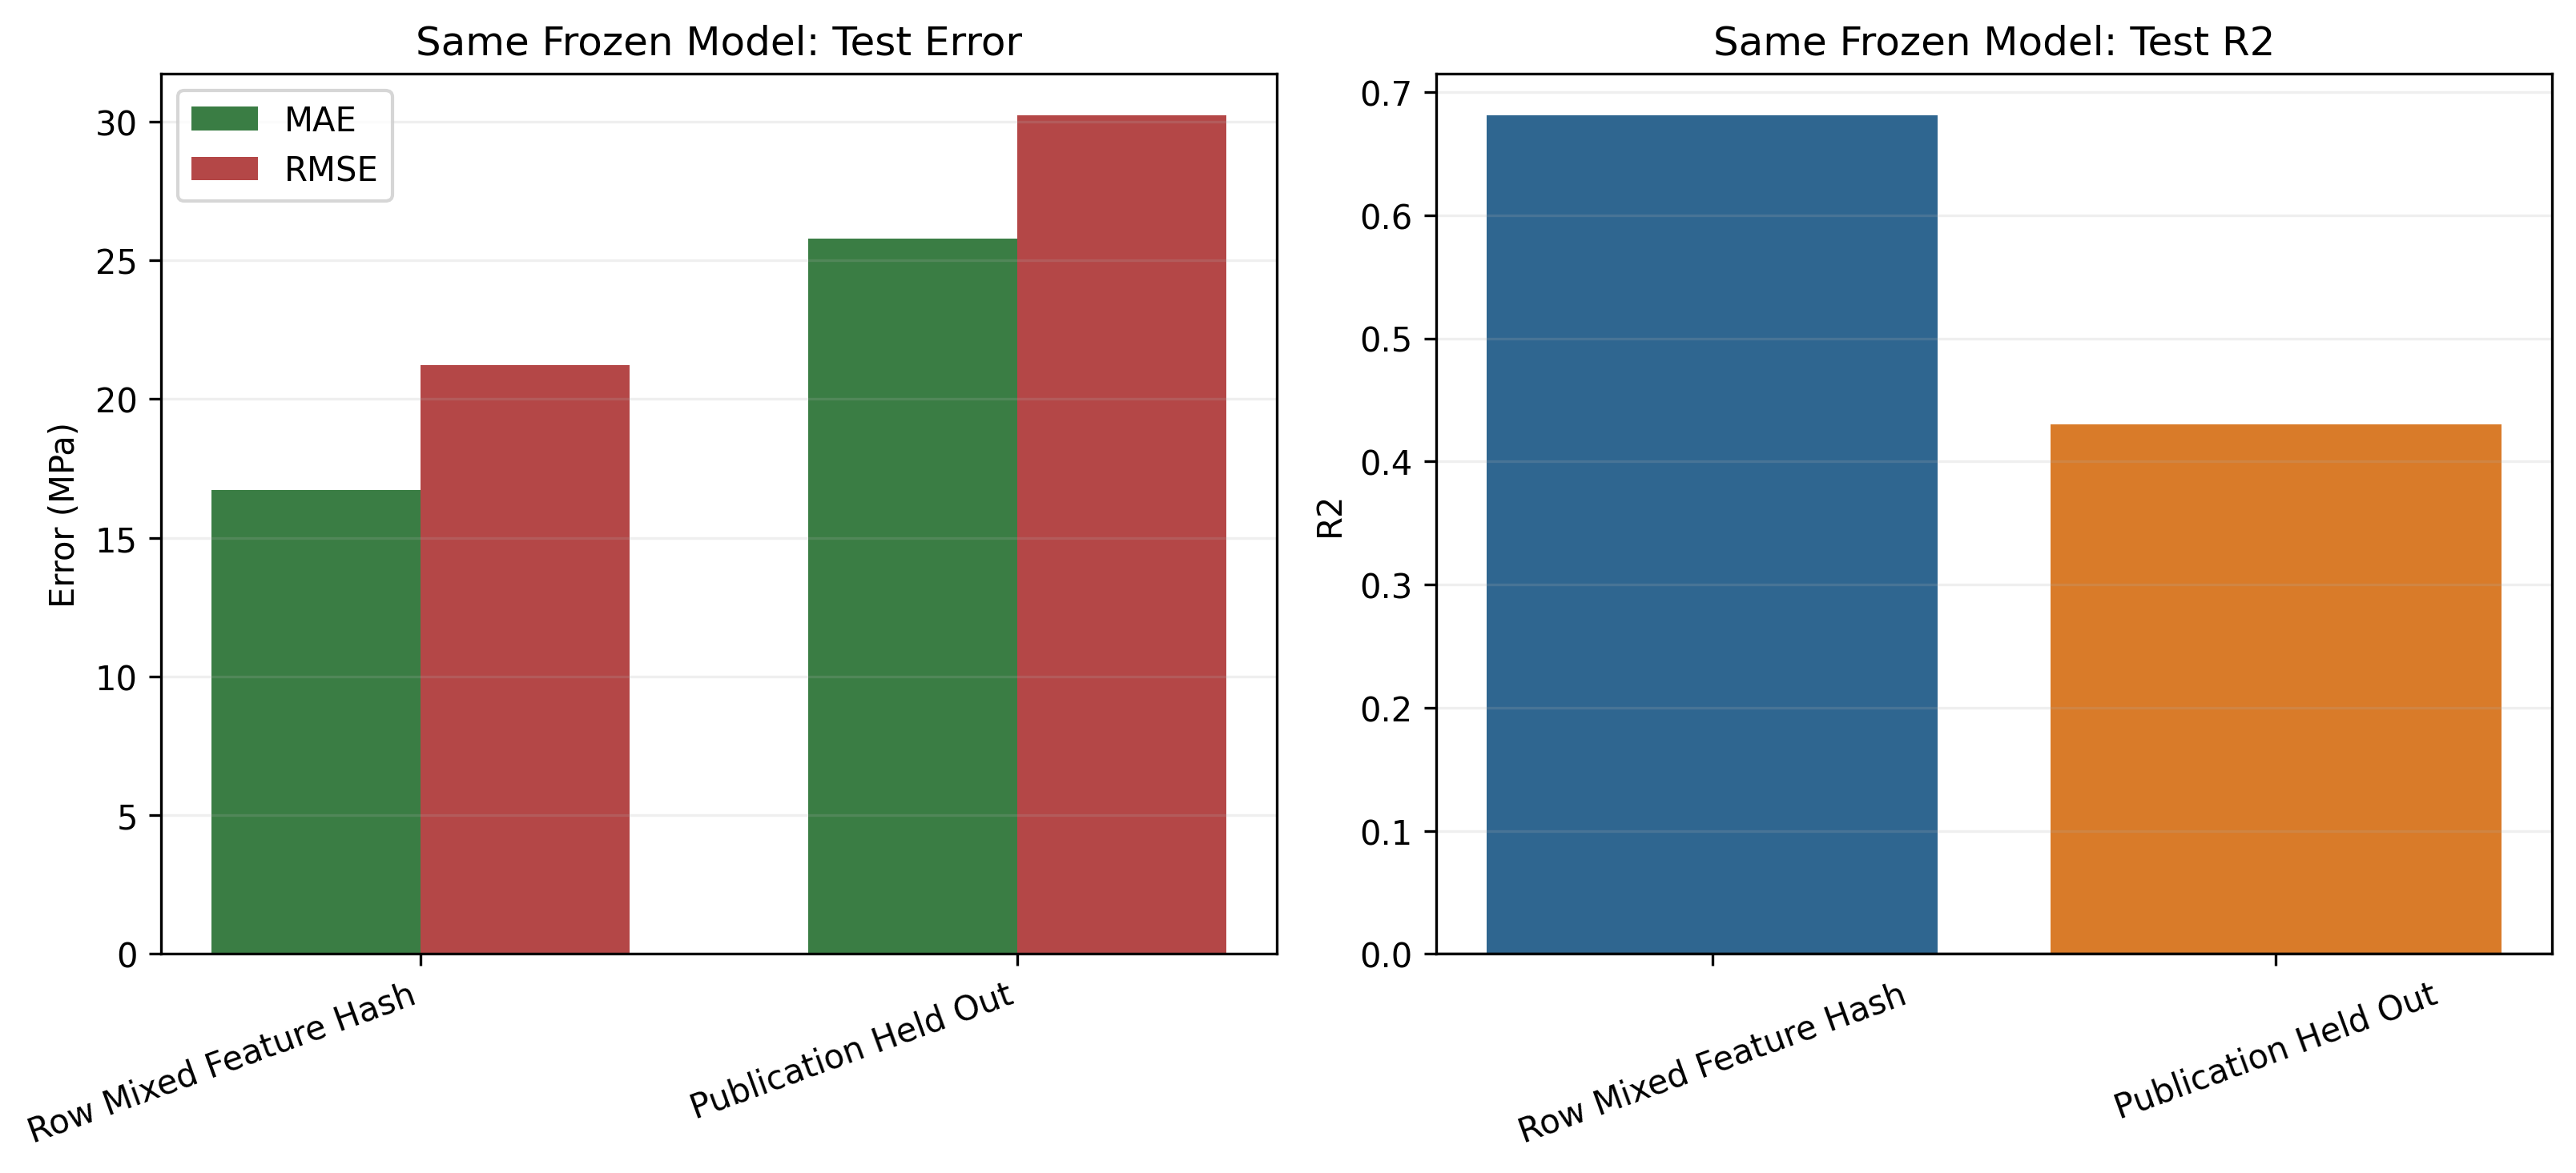
\includegraphics[width=0.86\textwidth]{report_assets/publication_generalization_gap.png}
\caption{Performance drop from row-mixed testing to publication-held-out testing.}
\label{fig:publication-gap}
\end{figure}

\subsection{Uncertainty and Calibration}
Prediction intervals were evaluated at the 90\% nominal level. This is important because a point prediction alone can hide how uncertain the model is on unseen publications.

\begin{table}[h!]
\centering
\small
\caption{Publication-held-out uncertainty results on the test set.}
\label{tab:uncertainty}
\begin{tabular}{llrrrr}
\toprule
\textbf{Method} & \textbf{Model} & \textbf{Coverage} & \textbf{Width} & \textbf{RMSE} & \textbf{$R^2$} \\
\midrule
Split conformal & Elastic Net & 0.894 & 94.46 & 28.49 & 0.493 \\
Native interval & Bayesian Ridge & 0.830 & 85.11 & 27.72 & 0.520 \\
Conformalized & Bayesian Ridge & 0.936 & 108.02 & 27.72 & 0.520 \\
Bootstrap & Elastic Net & 0.743 & 66.94 & 28.49 & 0.493 \\
Bootstrap conformalized & Elastic Net & 0.916 & 95.15 & 28.49 & 0.493 \\
\bottomrule
\end{tabular}
\end{table}

The conformal methods were closest to the intended 90\% coverage. The cost was wide intervals, roughly 95--108 MPa. This is a practical warning: the model can express uncertainty, but unseen-publication uncertainty is large.

\begin{figure}[h!]
\centering
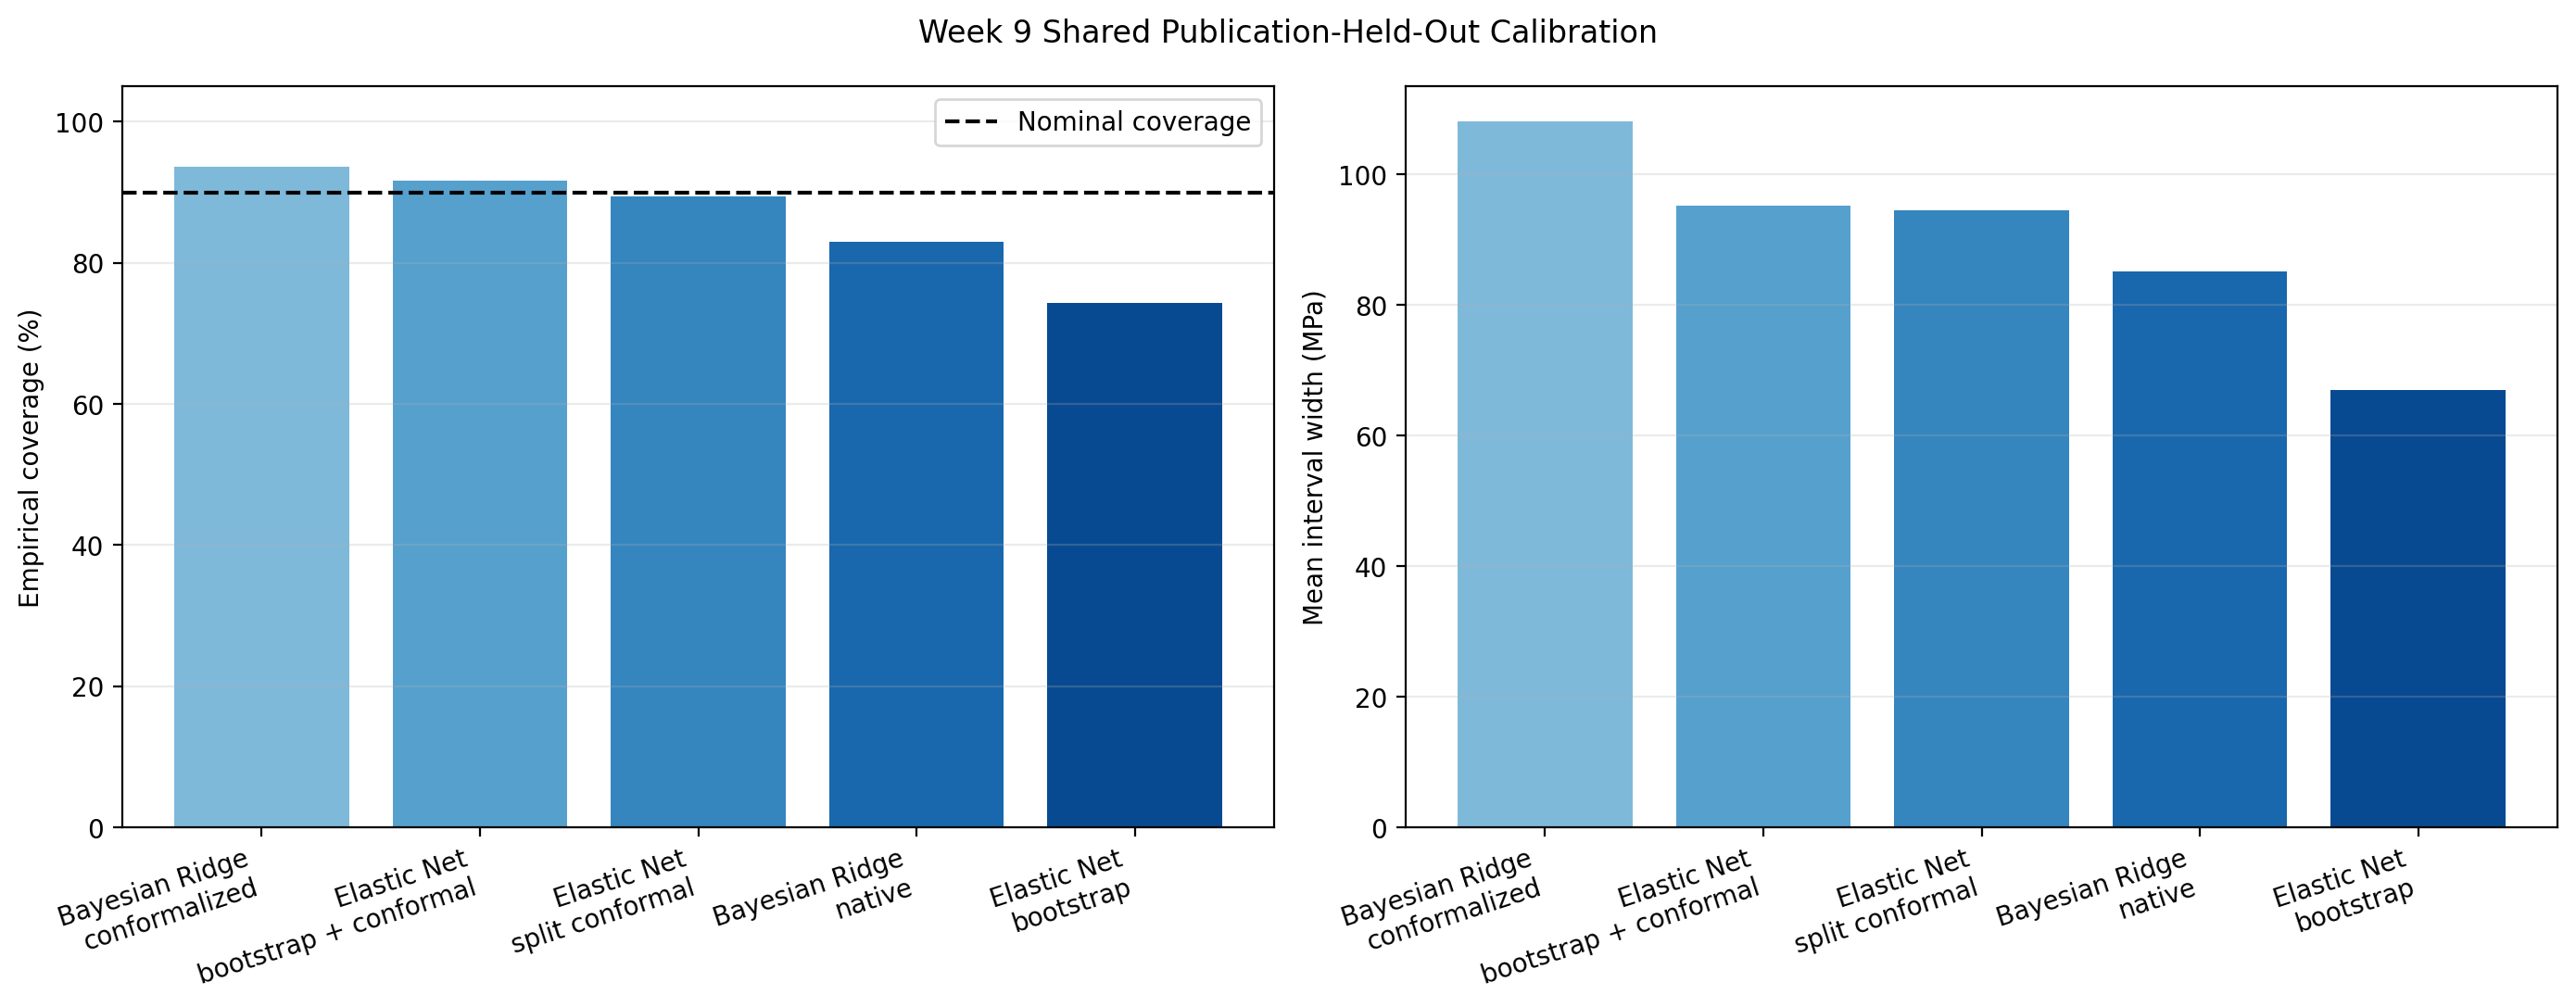
\includegraphics[width=0.82\textwidth]{report_assets/uncertainty_coverage_width.png}
\caption{Coverage and interval width for uncertainty methods on held-out publications.}
\label{fig:uncertainty}
\end{figure}

\subsection{Feature Attribution}
SHAP and permutation importance were used to check whether the model relied on physically meaningful groups.

\begin{table}[h!]
\centering
\small
\caption{Grouped feature attribution on the publication-held-out test set.}
\label{tab:attribution}
\begin{tabular}{lrrrr}
\toprule
\textbf{Feature Group} & \textbf{SHAP Mean} & \textbf{SHAP Rank} & \textbf{Permutation $\Delta$RMSE} & \textbf{Perm. Rank} \\
\midrule
Curing conditions & 13.31 & 1 & 8.52 & 1 \\
Fibers & 8.85 & 2 & 3.84 & 2 \\
Fillers and aggregates & 8.38 & 3 & 2.25 & 3 \\
Binders and SCMs & 7.32 & 4 & 0.86 & 4 \\
Water & 2.78 & 5 & 0.53 & 5 \\
Chemical admixtures & 2.34 & 6 & 0.25 & 6 \\
\bottomrule
\end{tabular}
\end{table}

Both attribution methods agreed on the top groups: curing conditions, fibers, and fillers or aggregates. The strongest individual feature was curing temperature. This is physically sensible because curing temperature changes hydration speed and strength gain. Fiber amount was also important, which matches the known role of fibers in UHPC.

\begin{figure}[h!]
\centering
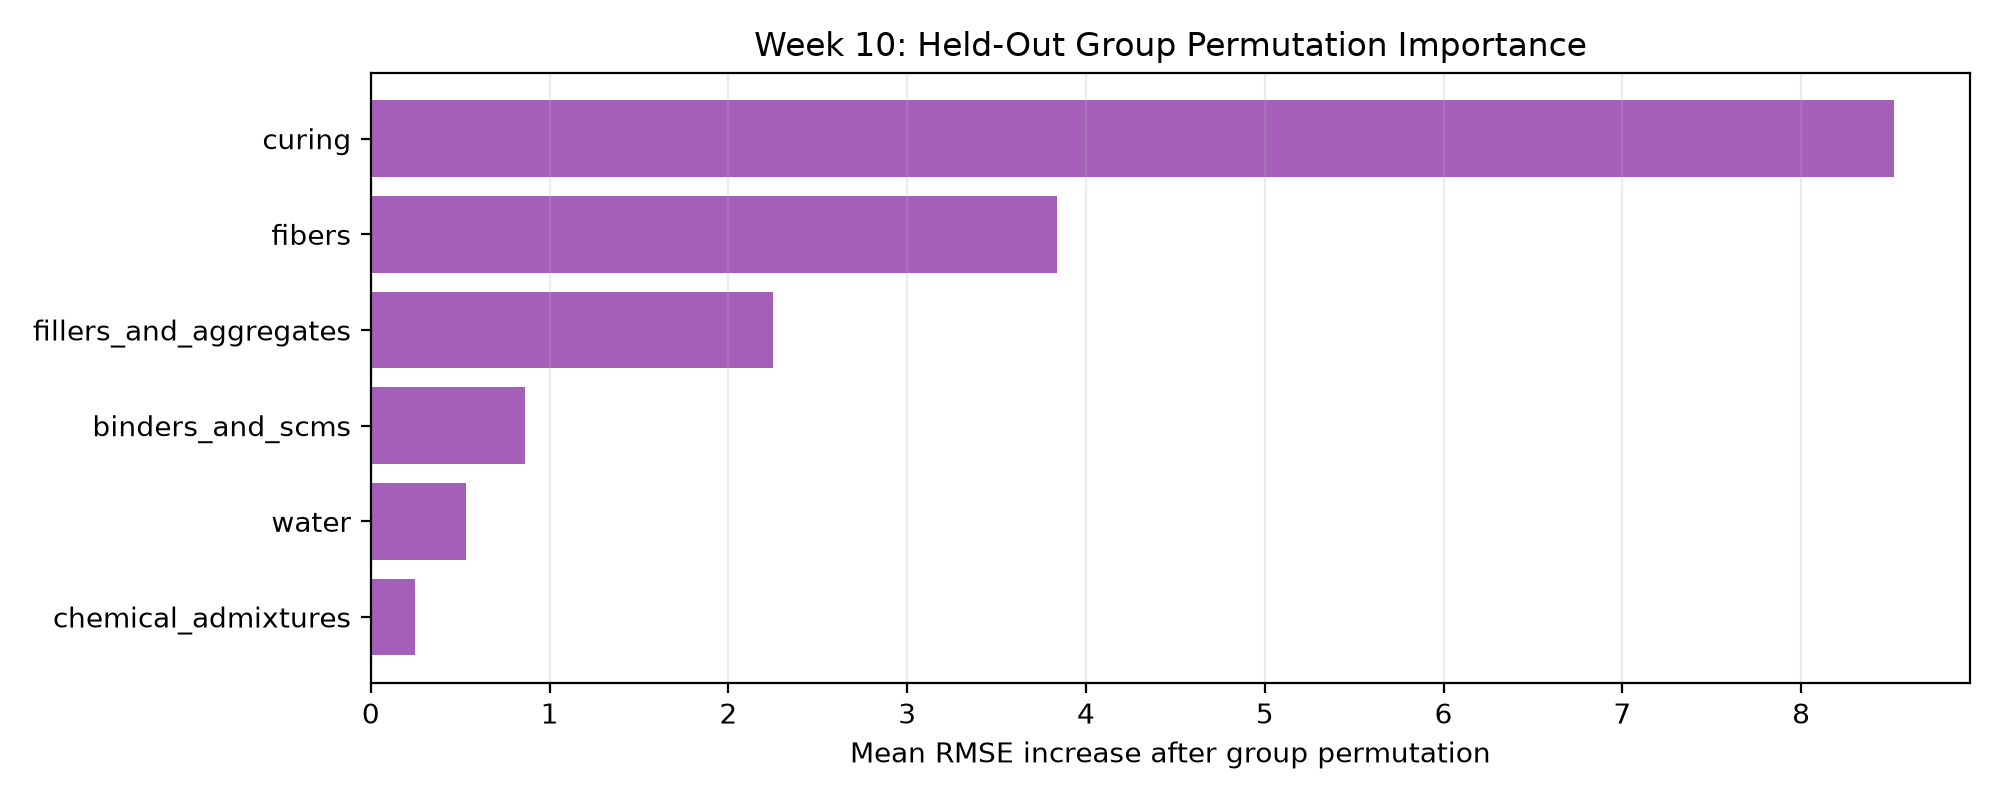
\includegraphics[width=0.78\textwidth]{report_assets/group_permutation_importance.png}
\caption{Grouped permutation importance after separating water and chemical admixtures.}
\label{fig:group-permutation}
\end{figure}

\section{Discussion and Conclusions}

The Linear Family performed very well on the UCI benchmark once polynomial and interaction features were used. This shows that simple models can be strong when the dataset is clean and the feature representation captures the main nonlinear effects.

For UHPC, the result was more limited. Row-mixed testing looked acceptable, but publication-held-out and LOPO testing showed a clear generalization problem. The model did not transfer equally well to new publications, which is realistic because UHPC data combines many laboratories, materials, and reporting styles.

The most reliable UHPC models were Bayesian Ridge and Elastic Net. Polynomial Ridge was powerful but unstable. The final interpretation was physically reasonable: curing, fibers, aggregates, and binders were important. However, the uncertainty intervals were wide, so predictions for unseen publications should be treated carefully.

\begin{thebibliography}{9}
\bibitem{uci}
I.-C. Yeh, Concrete Compressive Strength Dataset, UCI Machine Learning Repository, 2007.

\bibitem{yeh1998}
I.-C. Yeh, ``Modeling of strength of high-performance concrete using artificial neural networks,'' \textit{Cement and Concrete Research}, vol. 28, no. 12, pp. 1797--1808, 1998.
\end{thebibliography}

\end{document}
